
\graphicspath{ {mainmatter/Fiebrink_2007/} }
\title*{2007: Don't Forget the Laptop: Using Native Input Capabilities for Expressive Musical Control}
\titlerunning{Don't Forget the Laptop}
\author{Rebecca Fiebrink, Ge Wang and Perry R. Cook}
\authorrunning{Fiebrink et al.}

%\institute{Rebecca Fiebrink \at Department of Computing\footnote{The original affiliation of all authors was the
%Department of Computer Science at Princeton University, with Cook also affiliated
%with the Music Department there.}, Goldsmiths, University of London \email{r.fiebrink@gold.ac.uk}
%\and Ge Wang \at Center for Computer Research in Music and Acoustics (CCRMA), Stanford University \email{ge@ccrma.stanford.edu}
%\and Perry R. Cook \at Department of Computer Science (also Music) (Emeritus) Princeton University \email{jprc@cs.princeton.edu}
%}
%
%
\maketitle

\abstract*{We draw on our experiences with the Princeton Laptop Orchestra in a discussion on using the laptop's native physical inputs for flexible and expressive control. While we recognize the value of custom controllers, we argue that built-in laptop capabilities meet other needs, particularly in offering practical and creative benefits in a laptop ensemble setting. We discuss a variety of example instruments that use the laptop's native capabilities and suggest avenues for future work. We also describe a new toolkit for rapidly experimenting with these capabilities.}


\section{Motivation}
Music performed using laptops has a large and growing body of practitioners in
both academic and popular realms. Recent proliferation of software tools (PD \cite{Puckette:1996},
SuperCollider \cite{McCartney:1996}, ChucK \cite{Wang:2003}, also new uses for Perl \cite{McLean:2004}, Python, etc.) has
greatly reduced the barriers of expertise, time, and money required to create
music, opening the door to hobbyists as well as extending possibilities for
dedicated performance groups. Our experiences with the Princeton Laptop Orchestra
(PLOrk) \cite{Trueman:2006}, an ensemble of laptop meta-instruments, highlighted several issues
in creating live computer-mediated performances for such a group. Among these
issues are how to foster musical expression in a variety of pieces, how to create
pieces that musically engage the performers and audience, and how to support
composers in developing pieces for the ensemble, in addition to all the practical
concerns of maintaining an ensemble of laptops.


Drawing on this experience, we hope to contribute to the discussion surrounding
expressive and effective control interfaces as it pertains to collaborative
laptop performance in research/compositional environments as well as in less
formal contexts. In particular, we recognize that custom music controllers can be
highly useful, but experiences show they come with their set of hurdles. These
include exacerbating the long set up/tear down time, complicating transportation,
requiring expensive sensors or components and expertise in their construction and
maintenance, and presenting steep learning curves to players. Furthermore, in
ensembles such as PLOrk, many composers work with the players during rehearsals
to develop their pieces and associated interfaces. Thus, rapid experimentation,
familiarity with control interfaces, and reduced development and setup overhead
are often essential to the successful crafting of a performance work. The central
issue we address here is how to mitigate the problems custom controllers present
for such an ensemble, while allowing expressive and flexible control and
experimentation for a variety of pieces.

Fortunately, the innate capabilities of laptops themselves continue to present
new opportunities for control. Devices such as accelerometers and cameras are now
often built-in, and standard input methods such as keyboards and trackpads can be
used in innovative ways (i.e., other than for executing commands,
point-and-clicking, etc.). In the context of crafting instruments, the
self-contained laptop has several advantages. The difficulties associated with
custom controllers (e.g., cost, availability, portability) are less problematic. 
Laptops are ubiquitous, and it is easy to develop and distribute software
compatible with built-in components. They are easy to transport and require no
special maintenance and setup overhead compared with many customized standalone
controllers.

Although input devices such as keyboards and trackpads are simple and not
physically configurable, software flexibility presents unexplored possibilities
for using these devices in new and musically interesting ways. Additionally, the
aforementioned benefits of relying solely on built-in components contribute to
the smooth functioning and creative well-being of a laptop performance ensemble.
Therefore, we begin by positing that laptops themselves merit the continued
attention of musical interface designers and researchers. We present several
examples of using the laptop as input device, and we suggest additional means of
exploiting laptop capabilities. We also describe a new lightweight toolkit for
quickly experimenting with and utilizing several of the native input capabilities
of the laptop.

\section{Background}
\subsection{Previous Work}
Laptop music performance dates back as far as laptops themselves, but especially
began to take off in the 1990's.  Smoky clubs from Tokyo to Berlin, LA to New
York began to host nights dedicated to noise, glitch, infrasound, and other new
electro-acoustic genres afforded by the new powerful portable computers. Some
used commercial sequencing software, while others opted for more general-purpose
languages such as MAX/MSP or SuperCollider.  For those inclined to make more
traditional music, software programs such as ReBirth (emulating the Roland 606,
808, 303 and other drum/bass machines), and Reaktor (emulating a modular
synthesizer) became available \cite{Loubet:2000,Weidenbaum:2006}. Recently the practice of ``live coding''
has become more popular, in which the performer(s) actually program the computer
live, often projecting the screen \cite{Wang:2004}.

Many laptop performers have exclusively used the capabilities inherent in
laptops for music and other control tasks, even though they may not have
discussed the choice to forego a more customized control solution. Obviously,
keyboard and mouse are nearly always used to control GUIs such as patches, or
possibly to write code. In these cases, keyboard and mouse inputs translate into
onscreen operations, which then influence the music; we are interested in the use
of such devices wherein each key press, mouse gesture, or other physical
interaction is \textit{directly} musically meaningful.

For example, an innovative, though non-musical, use of a built-in laptop
capability is the ``SmackBook,'' where users can perform user interface
operations by physically hitting or tilting the laptop. Popularized in an
internet video \cite{Ellingsen:2006}, this clever ``hack'' uses the built-in sudden motion sensor
designed to protect the hard drive. We hope to transport this creative
resourcefulness into the musical domain.

\subsection{Context}
One driving philosophy of the NIME community is that controller design greatly
influences the sort of music one can make \cite{Cook:2001}. Our work in promoting simple,
standard controllers is not meant to contradict this belief. We are interested in
developing control methods in specific settings (e.g., laptop ensembles), and in
encouraging the community to consider all impacts of controller choice in
scenarios presenting practical limitations. Customization of controller to
musical task is desirable, yet so are availability, ease of use, development
time, and portability. In a real-world environment, these needs must be balanced
appropriately to maximize musicality, efficiency, and fun.

\section{Mapping Strategies}
In the following section, we describe several native laptop input capabilities
with case studies of their use in PLOrk performance. Much of the code used in
these pieces is included in our toolkit, which is discussed in Section 5.

\subsection{Keyboard}
While the decidedly discrete nature of the laptop keyboard makes it impractical
for some tasks, its form factor is optimized for small, fast, and precise finger
movements, and musical mappings might leverage the performer's existing typing
skills. For this reason, the keyboard can be a natural, if simple, musical
controller. In Wang's \textit{CliX}, performed by PLOrk, human operators type to
trigger sounds, which are synthesized, synchronized, and spatialized by their
laptops. Every key on the computer keyboard (upper- and lower-case letters,
numbers, and symbols) is mapped to a distinct pitch using the key's ASCII
representation, and when pressed, the laptop emits a clicking sound that is
synchronized through the ensemble to a common pulse. A human conductor
coordinates frequency range, texture, global spatialization, and timing.

The mapping is easily understood by players, who can immediately begin to make
sounds without practice. The ASCII-based layout makes it difficult to play
melodies but is sufficient for selecting relative pitch regions based on the
alphabet (for example, letters `U' through `Z' result in lower pitches than `a'
through `d').

In another set of pieces, keys are mapped to pitches in a fretboard-like
configuration, so notes and chords can be played with one hand with minimal hand
displacement (see Figure~\ref{fiebrink:fig:1}), leaving the other hand to operate a different
controller. This particular mapping was first used in Wang's \textit{Crystalis}
and later extended in Fiebrink, Wang, and Cook's \textit{Joy of Chant}.

\begin{figure}[t]
\begin{center}
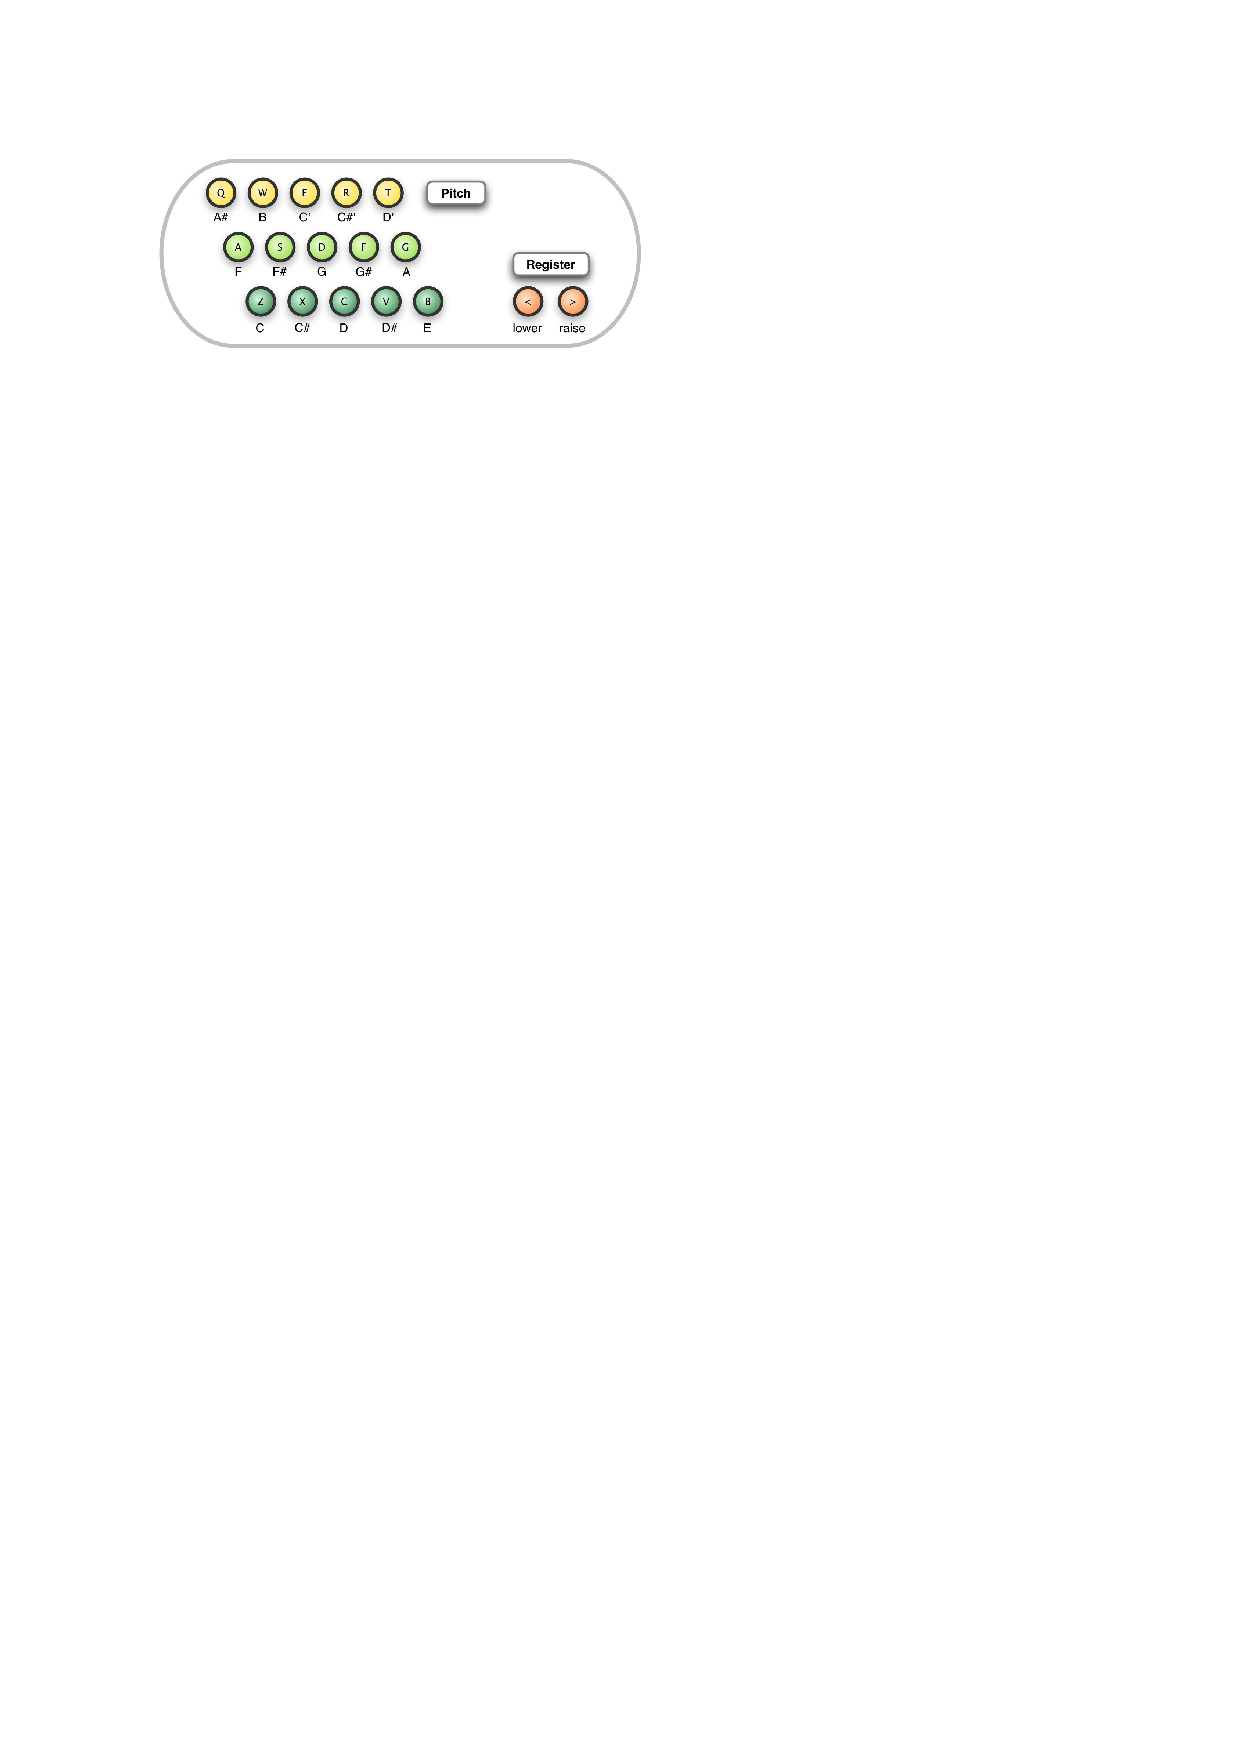
\includegraphics[width=\textwidth]{img-1-eps-converted-to.pdf}
\caption{Fret-based pitch selection.}
\label{fiebrink:fig:1} 
\end{center}
\end{figure}

Performers of \textit{Crystalis} follow the conductor to adjust pitch, density,
and volume, similar to \textit{CliX}, while controlling other parameters using
the trackpad (discussed in the next section). In contrast, \textit{Joy of Chant}
requires performers to use one hand to select specific pitches in unison from a
score, while the other hand controls singing synthesis parameters via a standard
joystick. \textit{Joy of Chant} extends the pitch selection keys rightward to
include the entire keyboard. Mappings of both pieces extend the pitch range by
providing means to shift registers in octave increments. In both cases, the
performers found the keyboard interface easy to use and were able to perform
after a few rehearsals.


Compared to the ASCII-based mapping, the fret-like mapping makes it easier to
play melodies; players need only remember the physical locations of pitches and
not of the letters. The letters can be notated in a score to help players learn
the music and the mapping (see Figure~\ref{fiebrink:fig:2}).

\begin{figure}[t]
\begin{center}
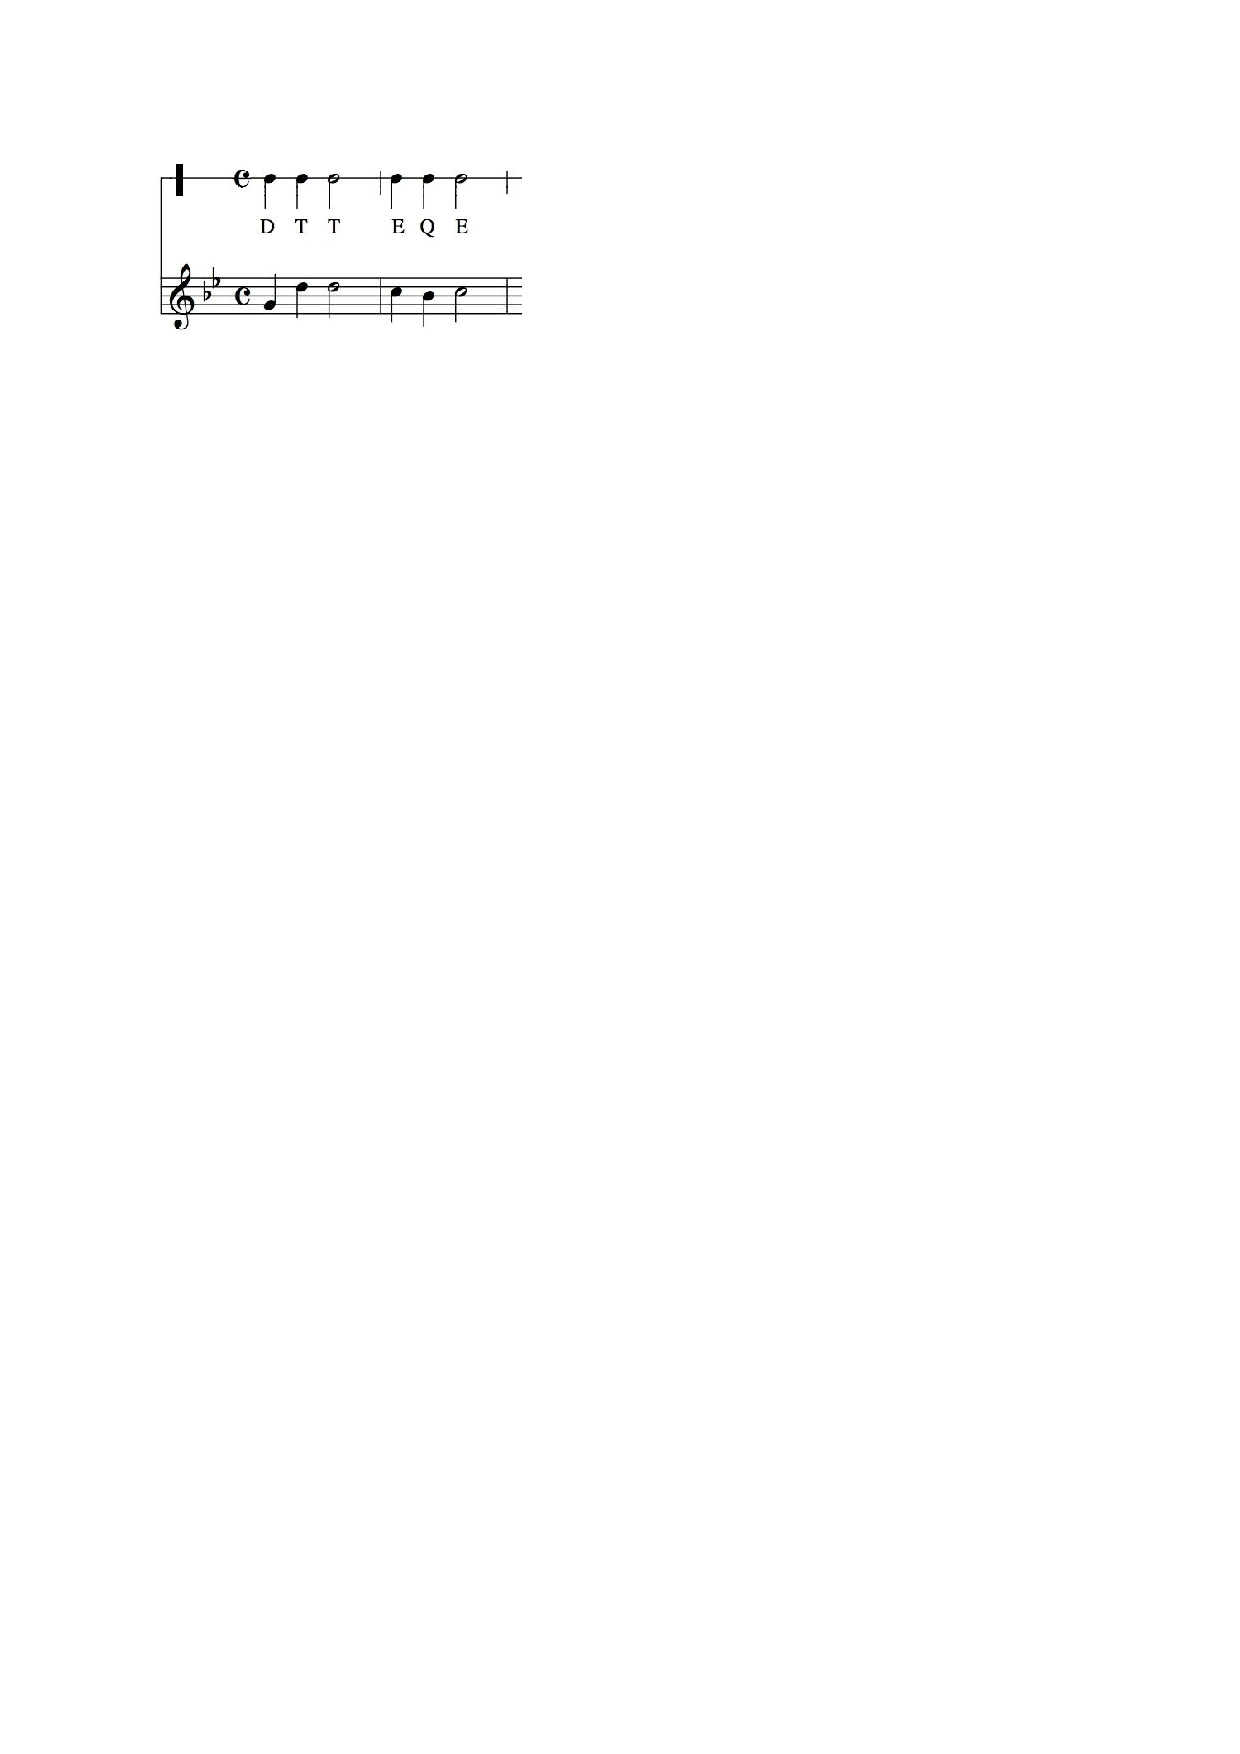
\includegraphics[width=178pt]{img-2-eps-converted-to.pdf}
\caption{Joy of Chant score (top) with traditionally transcribed equivalent
(bottom).}
\label{fiebrink:fig:2} 
\end{center}
\end{figure}


\subsection{Trackpad}
Looking past its use as pointing device, the ability of the trackpad to track
two-dimensional motion offers a wide array of mapping strategies. One of the most
heavily researched HCI devices \cite{Zhai:2004}, the modern trackpad offers fine-grained,
low-latency sensitivity with tactile and visual feedback.

In \textit{Crystalis}, players ``bow'' the trackpad by varying location and
speed to put ``energy'' into a synthesis model, in tandem with keyboard pitch
control. This mapping involves capturing finger motion (as relative x and y
position updated at interactive rates), which is low-pass filtered (2nd order
Butterworth with 10 Hz cutoff). This signal is then passed into a leaky
integrator (one-pole low-pass filter) that generates an envelope with a smooth
attack and gradual release, which is in turn multiplied with the source signal
(wind-like sounds or a banded waveguide model). Moving the fingers quickly tends
to result in louder and more energetic sounds. Bowing in different directions
places sound into particular audio channels. Physical finger patterns directly
correspond to audio/spatial patterns (see Figure~\ref{fiebrink:fig:3}). For example, making a
circular pattern on the trackpad will move the sound smoothly around the output
channels. The tight coupling between finger location and spatialization and
between player effort and sound energy make this a natural mapping.

\begin{figure}[t]
\begin{center}
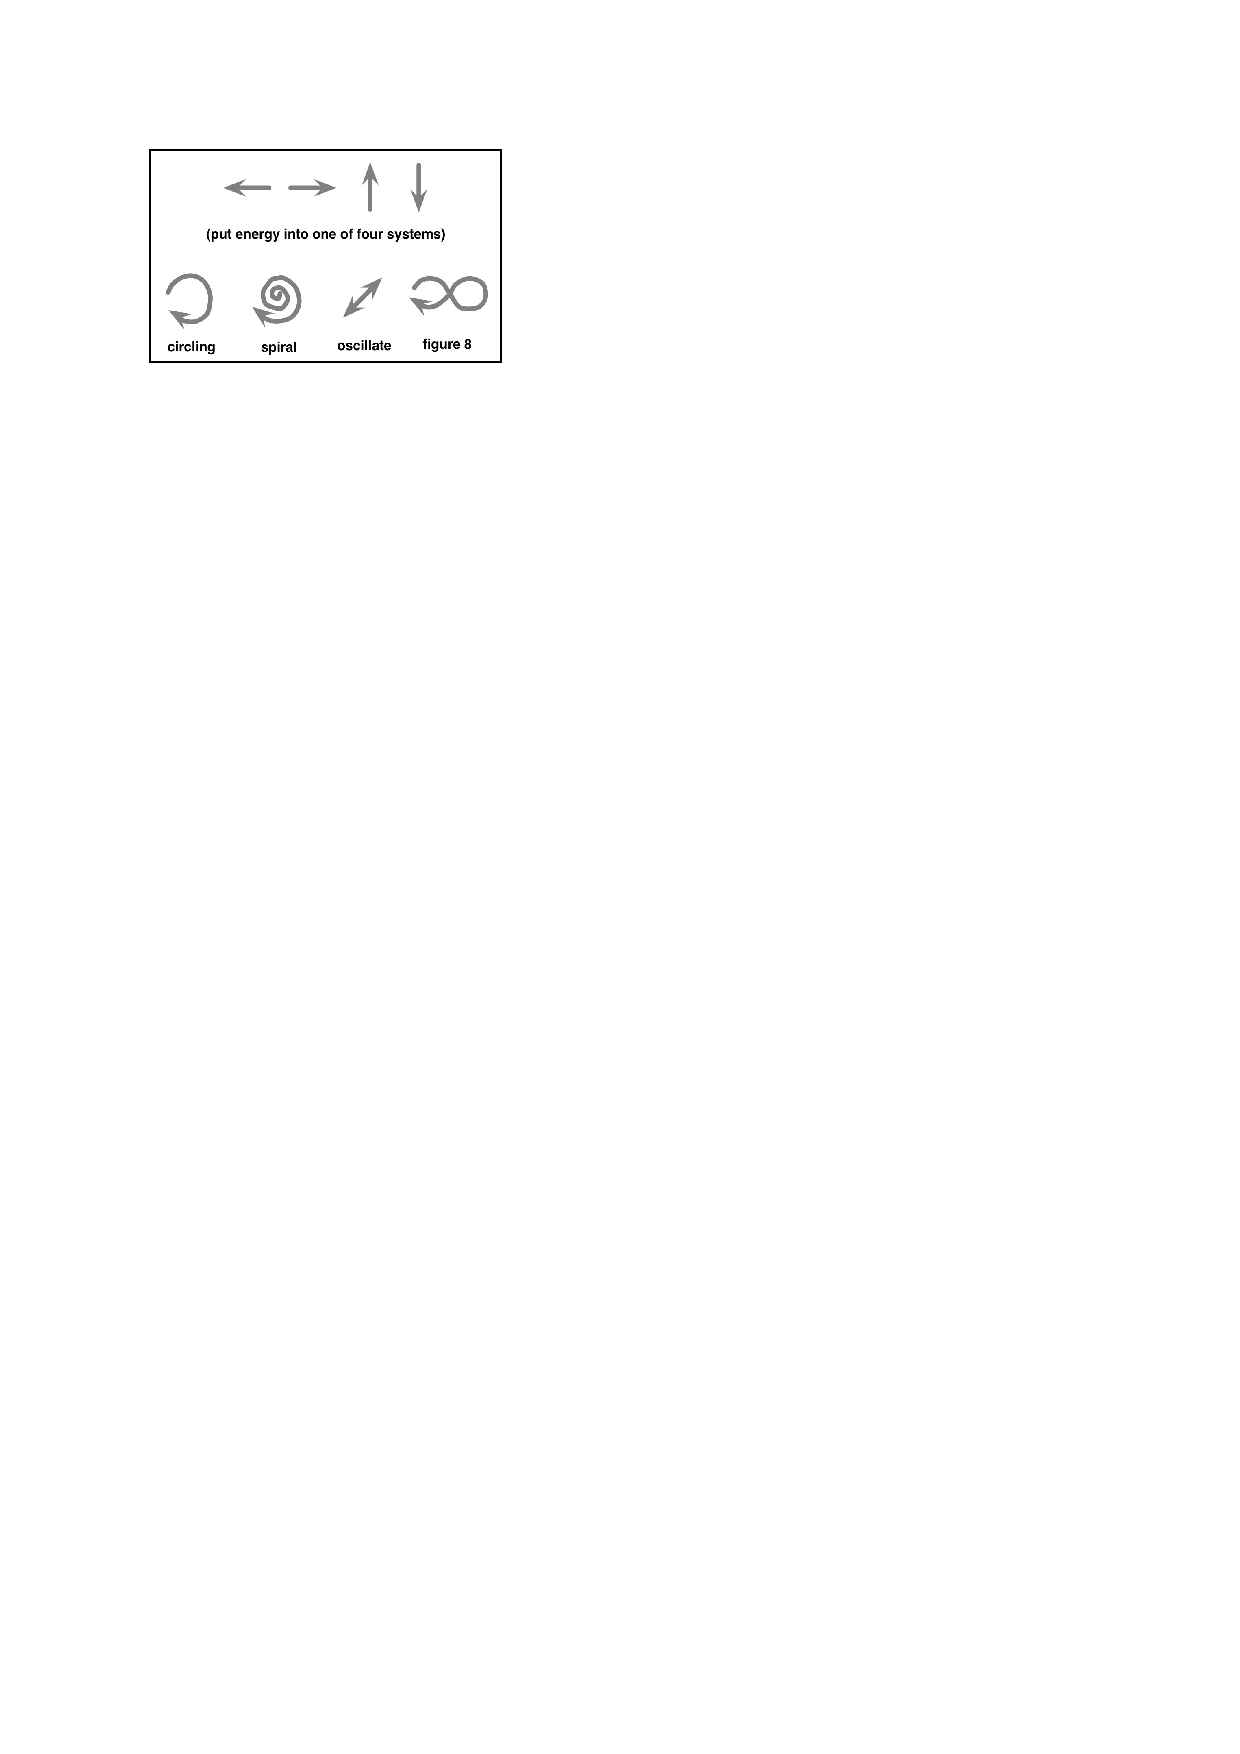
\includegraphics[width=70mm]{img-3-eps-converted-to.pdf}
\caption{Trackpad bowing motions.}
\label{fiebrink:fig:3} 
\end{center}
\end{figure}

\subsection{``Smack-sensing''}
A less commonly used input capability is the accelerometer-based motion sensor
found in many laptops. In Fiebrink's \textit{Smacking Music}, PowerBook laptops
are used as ``acoustic'' percussive instruments to perform Steve Reich's
\textit{Clapping Music}. Performers hit their laptops with hands or other objects
to produce the auditory component of the piece. The built-in sudden motion sensor
is polled by a software application, and motion events surpassing a certain
amplitude threshold are registered as ``smacks.'' In response to each smack, the
laptop display is modified, producing a synchronous visual accompaniment.

The piece is performed with any number of people, separated into two groups, one
for each part of the original score. Laptop screens face the audience, who
observes both smacking gestures and laptop screens. Performers are encouraged to
hit the laptop wherever and however they like. The laptop motion sensor is
suitably sensitive that little force is required (e.g., tapping the laptop base
with a pen). Fortuitously, the motion sensor continues to perform its intended
role of protecting the laptop hard drive from harm throughout the piece,
minimizing the risk posed to the computer by the performer. The experiences of
performing and observing this piece are quite novel and entertaining.

The sudden motion sensor output provides absolute tilt information in three axes
dozens of times per second. Other physical stimuli, such as shaking or tilting,
can also easily be captured, conditioned, and used as control parameters.

\subsection{Laptop Speaker and Microphone}

While far below the quality of those typically used in laptop performance, the
laptop's integrated microphone and speakers can themselves be used as novel
input/output devices. Matt Hoffman's \textit{Breathalyzer?} requires performers
to blow directly into the laptop's microphone. The sound of the piece is
band-pass filtered computer generated noise; when the noisy input of the
performer's breath is detected, the center frequency of the bandpass filter is
changed. The piece takes form as performers influence their filters as a
coordinated ensemble.

In this piece, the microphone senses the presence or absence of breath. The use
of microphone input can easily be extended to track continuous variables, such as
the amplitude envelope of the breath, for other mappings. The quality of the
laptop microphone is satisfactory for capturing this coarse control data.

While the input methods addressed in this section can be used with external
speakers to produce high-quality sound output, it is also interesting to consider
their use in spontaneous, highly portable settings. In fact,
\textit{Breathalyzer?} is one of a series of PLOrk pieces, \textit{Small Sound
Sketches}, composed to use the laptop speakers (and humans) as the sole means of
output (this is as close as we can get to ``PLOrk Unplugged''). This constraint
led to several creative approaches to ``portable'' music making, demonstrating
that this can be an interesting ``extreme'' approach to allow maximally portable
laptop ``jam sessions.''

\section{Other Input Methods}

\subsection{Networking}

Today's laptop comes standard with capabilities for easily creating ad hoc
wireless networks, without the need for extra hardware. Furthermore, developing
software to communicate with other laptops on a network is quite straightforward,
particularly when using established protocols such as Open Sound Control \cite{Wright:1997}.
Several PLOrk pieces have used networking as an integral component. In
\textit{CliX}, for example, a machine ``conductor'' synchronizes and quantizes
the sounds triggered by each player's keyboard by emitting periodic pulses via
OSC, leveraging the computer to augment the degree of control offered by the
keyboard. In Fiebrink and Wang's \textit{PLOrk Beat Science}, five networked
laptops act as a distributed sound bank, and a player at one machine can trigger
sounds on other machines to create spatial patterns.

\subsection{Webcams}

The video camera has been used as a musical input device in the past, for
example in the Mouthesizer \cite{Lyons:2001a}. As many laptops begin to be shipped with built-in
webcams, video and photo input capabilities are increasingly available for use in
laptop music. Future work for our toolkit includes integrating webcam
functionalities such as raw video capture and basic image analysis, so users can
integrate live input, such as the Mouthesizer, into any performances.

\subsection{Don't Rule Anything Out}

Even less obvious channels for communicating ``information'' to a laptop might
be used for musical control. Other increasingly standard laptop features include
Bluetooth and remote control (e.g., MacBook and Dell Inspiron series). One might
devise pieces to take advantage of even the most trivial laptop controls, such as
buttons for power, volume, brightness, etc. Operating system-specific tools such
as AppleScript can also be used effectively to access and control basic system
features. While latency, bandwidth, and other issues may limit the usefulness of
such controllers, we believe that mundane features may still have musically
interesting applications.

Laptop technology may soon grow to include yet more varied and promising
interfaces for control. A 2005 Apple patent application describes a ``mechanical
overlay'' touch-sensitive interface, which would integrate into the laptop
hot-swappable mechanical controllers, such as knobs, sliders, joysticks, and
piano-like keyboards \cite{Huppi:2005}. If such technologies come to be standard, these
controllers would open up even more opportunities for laptop-contained control
with the aforementioned benefits of portability, low maintenance overhead, and
ubiquity. Musical interface designers should stay informed of such developments
with an eye toward their obvious and non-obvious potential uses in music.

\section{A new Toolkit}
We have assembled a publicly available toolkit, the Small Musically Expressive
Laptop Toolkit (SMELT), to facilitate rapid development and experimentation using
some of the control capabilities mentioned above.\footnote{\url{http://smelt.cs.princeton.edu/}} This toolkit contains a collection of C source
code modules and examples in the ChucK programming language. Many of the tools
arise out of our previously discussed work with PLOrk, and are summarized in
Table 1 below. 

We hope that releasing this toolkit will encourage other performers, composers,
and researchers to similarly make available their code for capturing laptop
inputs for novel musical expression. Our vision is that these tools might join
the standard palette used to craft collaborative laptop music performance. A
critical mass of ubiquitous, easy-to-use code can encourage willing experimenters
to make more music together with their laptops, while continuing to ponder and
refine the use of laptop inputs for musical ends.

\begin{center}
\begin{table}[t]
\ra{1.4}
\setlength{\tabcolsep}{12pt}
\caption{Toolkit components}
\vspace{3pt} \noindent
\begin{tabular}{p{40pt}p{45pt}p{70pt}p{60pt}}
\toprule
\textbf{Input}     & \textbf{Language}  & \textbf{Description}  & \textbf{Examples} \\
\midrule  
Keyboard & ChucK & {\small ASCII and fret-like pitch selection} & \textit{CliX}, \textit{Crystalis}, \textit{Joy of Chant} \\
Trackpad & ChucK & mouse and trackpad bowing & \textit{Crystalis}\\
Motion & C, ChucK & {\small motion sensing and signal conditioning code, user API} & \textit{Smacking Music} \\
Mic & ChucK & breath control & \textit{Breathalyzer?} env. follower \\
\bottomrule
\end{tabular}
\end{table}
\end{center}

\section{Concluding Remarks}

Custom controllers play a necessary role in facilitating expressivity and
creativity in performance of new music. However, certain rehearsal, composition,
and performance paradigms can benefit from the low overhead, ease of use, and
availability of the native laptop input capabilities. Furthermore, creatively
exploiting these capabilities can lead to interesting musical possibilities. In
our experiences with the Princeton Laptop Orchestra, we have found the use of
native laptop inputs to support the development of new compositions in a group
setting, and to be effective in performing a variety of compositions. We believe
that laptop controls are not only useful in PLOrk-like laptop ensembles and
chamber music settings, but they also encourage spontaneous and informal musical
collaboration. Both paradigms can benefit from reducing barriers of cost,
overhead, learning curve, etc. while preserving a variety of control options. The
laptop is a popular and evolving instrument that can be played anywhere, anytime,
by anyone. We hope that our work, and that of others interested in musical
interfaces, can increase the expressive capabilities of laptops by calling
attention to and writing code in support of the laptop's natural capabilities for
novel musical ends.

\begin{acknowledgement}
Our thanks to the Princeton Laptop Orchestra, Dan Trueman, Scott Smallwood, Matt
Hoffman, and Spencer Salazar.
\end{acknowledgement}

%\input{referenc}

\section*{Author Commentary: Remembering the Laptop: Looking Back at SMELT}
\paragraph{Rebecca Fiebrink, Ge Wang, and Perry R. Cook}

When we wrote this paper in late 2006, the Princeton Laptop Orchestra had existed as a performing and teaching ensemble for over a year. We had each written pieces for PLOrk and were becoming familiar with the musical and practical consequences of different types of physical inputs in an educational undergraduate ensemble. We had also been composing and experimenting in a graduate seminar on ``laptop chamber music,'' using smaller groups and more lightweight setups. Reflecting together on our favorite pieces for these ensembles, we realised that many of the instruments we had been building with the laptops had an intrinsic physicality that was more akin to controller-based performance than point-and-click GUI control. We identified the common principles that we felt made these instruments successful, we packaged up some example code to make it easy for others to build similar instruments, and this paper and the Small Musically Expressive Laptop Toolkit (SMELT) were born.

Eight years later, SMELT is still a constant presence in our lives. Although our paper doesn't explicitly consider the educational benefits of this approach, SMELT has hugely impacted our teaching. SMELT is our go-to tool to quickly demonstrate to new students the musical possibilities (and fun!) of using laptops to play music, without the need for specialised hardware or extensive computer programming skills. Hundreds of our own students---from Princeton PhDs to 8-year-old workshop attendees---have used SMELT to build their first instruments. The three of us still often reach for SMELT when we sit down to write code for a new laptop instrument, because it allows us to immediately experiment with new interactions with sound.

We've made good on our stated plans to continue to explore other native laptop input capabilities, though we have not integrated them formally into the SMELT toolkit. Fiebrink has made extensive use of laptop webcams in performance and teaching; for instance, performers in her laptop orchestra piece Blinky (2009) control sound using flashlights captured by the webcam. Cook has often used the accelerometer as a tilt sensor in pieces for PLOrk, SLOrk, LOrkAS, and others. In a 2008 Stanford Laptop Orchestra piece by Wang's students (\emph{20} by Kyle Spratt and Adnan Marquez-Borbon), performers adjust the angle of the laptop screen hinges to expressively control audio feedback between 20 laptops. 

Our experiences continuing to explore native input capabilities also suggest some caveats to add to the original paper, perhaps best summarized as ``Don't forget the laptop, but don't count on it, either!'' Our methods for obtaining sensor data from laptops have often relied on unpublished APIs which break when operating system or hardware versions change. Newer laptops with solid-state hard drives need no sudden motion sensor, leaving us without native smack or tilt sensing; Cook has resorted to taping an iPhone to his new laptop to use its accelerometer (via TouchOSC) in demos and performances!

In fact, the dramatic changes in computing hardware since 2007 also drove one of the most important and unanticipated directions of our work: extending this same design ethos beyond the laptop. Apple introduced the iPhone a few weeks after the NIME 2007 conference. Shortly thereafter, Wang started the Stanford Mobile Phone Orchestra (MoPhO) and co-founded mobile app company Smule (with whom Cook and Fiebrink have also worked). Many MoPhO pieces and Smule apps co-opt native mobile phone input capabilities in expressive ways that echo our previous use of laptop inputs. For instance, the phone microphone is used as a breath sensor in Sonic Lighter and Ocarina \cite{Wang:2014}---two of the first Smule apps---along with accelerometer and multitouch as a physical input. An early version of the Magic Fiddle iPad app used the touch screen to track finger positions as well as chins---requiring players to hold the iPad under their chins like a violin. Through these apps, over 125 million people worldwide have used the phone as a physical controller to expressively perform digital music.

Thus, today we might characterise this paper not as a paper about the laptop, but rather a paper that is essentially about a design ethos of taking whatever inputs and sensors happen to be available and thinking as broadly as possible about their interactive affordances. This ethos recognises that physicality and extreme convenience can coexist, and together have a tremendous positive effect on instrument building, composition, performance, and teaching. Furthermore, taking familiar input capabilities and co-opting them in unfamiliar ways can imbue expressive musical interactions with a sense of playfulness, something we try to cultivate in much of our music-making and teaching.

\section*{Expert Commentary: Developing a Digital Virtuosity}
\paragraph{Andrew R. Brown}

The article, ``Don't forget the Laptop'' by Fiebrink, Wang and Cook, focuses on using a laptop computer's native user interfaces for expressive control of music in laptop ensemble performance. This topic was foreshadowed by others in the computer music community \cite{Schiemer:2005}, but is perhaps of even more interest now, 8 years after publication, than when it was written. There is currently a proliferation of commercial physical controllers and DIY solutions for electronic music performance. 

In the article, Fiebrink, Wang, and Cook argue that external controllers can impose various logistical hurdles that justify the serious consideration of the musical affordances of built-in interfaces; such as qwerty keyboards, track pads, accelerometers, light sensors, microphones, video cameras and wireless networking. The laptop is still quite dominant in music production and performance but is being joined by an increasing array of mobile computing devices that feature an even larger array of native interface sensors. These sensor-rich mobile devices further amplify the opportunities for expressive musical interaction with technology \cite{Tanaka:2012}.

At the heart of the utilization of these native interfaces is the challenge of mapping data from them to musical ends when the interfaces were not designed with musical expression in mind \cite{Hunt:2003}. The authors survey various laptop interaction strategies employed by them and their colleagues in the Princeton Laptop Orchestra (PLOrk). These strategies include using the keyboard to trigger events, using the trackpad to activate events and vary parameters, and using the accelerometer to recognize percussive gestures. They introduce an open-source library of ChucK code that has been developed to facilitate these laptop interaction strategies.

Laptop computers are used in performance in various ways; as playback devices: as the basis for remixing playback streams, for the control of live-algorithms---as is typical in laptop ensembles---to live coding performances where text becomes both the medium of musical representation and the qwerty keyboard the primary control interface \cite{Brown:2006}. Each of these performance situations make different demands on the laptop as musical instrument which, in turn, conditions our shared struggle to balance the design of musical controls with the design of musical outcomes.

It is helpful that investigations, such as those reported in this article, underscore our need to explore the use of technologies as musical instruments and our work at developing techniques for effective music production that strive to achieve \lq data virtuosity\rq \cite{Tobias:2012}. Tobias' concept of data virtuosity in digital music making highlights an expansion in expertise from gestural techniques on acoustic instruments to skills that include the collection, mapping and utilisation of data from user interfaces. This expansion of the digital musician's skill set results in a need for persistent exploration and development of reasonably stable electronic instruments, such as laptop computers, that can lead to well-honed techniques and musically sophisticated outcomes.

This article provides useful insights into how the ongoing challenges of musical expression in live performance reappear at each stage in technological progress; in this case in the context of laptop orchestras that arose naturally at a time when laptop computing was at its most dominant. This approach to designing musical interactions with commodity technologies that are ready-to-hand is one that is increasingly appropriate in an age of rapid technological revolution and especially prevalent in the \lq maker\rq and \lq ubiquitous music\rq communities.
